\documentclass[11pt]{article}

\usepackage{fontspec}
\usepackage{polyglossia}
\setmainlanguage{english}
\setotherlanguage{arabic}
\newfontfamily\arabicfont{Tahoma}[Script=Arabic]

\usepackage[margin=1in]{geometry}
\usepackage{graphicx}
\usepackage{booktabs}
\usepackage{caption}
\usepackage{xcolor}
\usepackage{hyperref}
\hypersetup{colorlinks=true, linkcolor=blue, urlcolor=blue}

\title{How Capable Is Qwen3.5 at OCR?\\
\large A Look at English and Arabic Book Scans}
\author{}
\date{}

\begin{document}
\maketitle

\section{Introduction}

I wanted to find out how far I could push Qwen3.5 as an OCR reader --- not because it's
built for that job, but because it's a vision-language model I could run entirely on my own
machine, and I was curious whether that would be good enough. My plan was simple: feed it
scanned pages from a few different books, in two different scripts, and check its
transcription word-for-word against a text I'd verified by hand.

Getting even this far took some working around. I picked Qwen3.5 over Qwen2 because it's
simply the stronger model --- a newer generation with better reasoning and multimodal
ability --- and it was still something my machine could run locally at a moderate pace.
That didn't make it fast: even with a capable-enough setup, individual pages still took
several minutes to process. It was a balance between running the strongest model I
reasonably could and still getting results back in a workable amount of time.

The test set: two different scans/editions of Aristotle's \emph{Nicomachean Ethics} in
English, and one Arabic-language biographical work,
\textarabic{فريدة الدهر في طبقات قراء مصر} (Volume 1). Every OCR result below is checked
against a hand-verified transcription of the same page.

\section{How Accuracy Is Measured}

Each result is scored three ways:

\begin{itemize}
    \item \textbf{Word Error Rate (WER)} --- out of all the words in the correct text, what
        percentage don't line up with what the model produced? This is the most intuitive
        number: it's roughly ``how many words would I have to fix by hand.'' Lower is
        better.
    \item \textbf{Character Error Rate (CER)} --- the same idea, but measured letter by
        letter instead of word by word. In principle it's a finer-grained version of WER.
    \item \textbf{Overall Similarity} --- a general string-similarity ratio between the OCR
        output and the correct text.
\end{itemize}

One warning about CER and Similarity, which shows up repeatedly below: both are computed by
lining up the two texts character-by-character, and that alignment can fall apart badly when
just a few words get reordered or reworded --- even if the surrounding text is almost
perfect. So a page can score a rough CER while still being highly readable and mostly
correct. WER is the number I trust most in this report; CER and Similarity are included for
completeness, but should be read with that caveat in mind.

\section{Aristotle --- Edition 1 (Older Translation)}

\begin{center}
    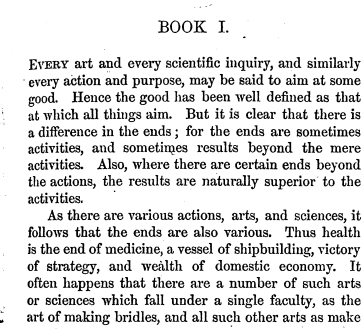
\includegraphics[width=0.85\textwidth]{aristotle1/page1.png}

    \bigskip
    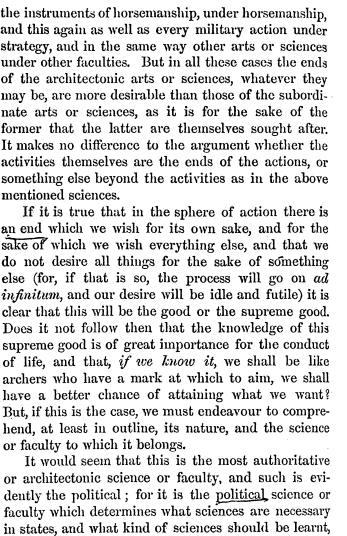
\includegraphics[width=0.85\textwidth]{aristotle1/page2.png}

    \bigskip
    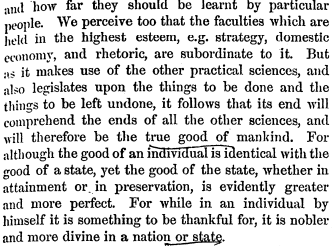
\includegraphics[width=0.85\textwidth]{aristotle1/page3.png}

    \captionof{figure}{Aristotle, Edition 1 --- an older, archaic-style translation.}
\end{center}

\bigskip
\begin{center}
    \begin{tabular}{lr}
        \toprule
        Metric & Value \\
        \midrule
        Word Error Rate      & 11.99\% \\
        Character Error Rate & 65.81\% \\
        Overall Similarity   & 33.42\% \\
        \bottomrule
    \end{tabular}
\end{center}
\bigskip

About 88\% of words came back correct. Most of what's wrong is trivial:

\begin{itemize}
    \item \textbf{Small word swaps:} ``at'' read as ``with''; ``Is'' read as ``Does.''
        Wrong, but harmless.
    \item \textbf{Line-break hyphenation:} words split across a line break came through with
        a stray space, e.g.\ ``subordinate'' as ``subordi- nate,'' ``comprehend,'' as
        ``com- prehend,''.
\end{itemize}

But a few errors go further than simple misreading --- the model rewrites entire clauses
into more modern, fluent phrasing instead of transcribing what's actually printed:

\begin{itemize}
    \item The original reads \emph{``\dots{}it must of the ends of all the other
        sciences\dots{}''} --- an awkward, archaic construction. Qwen's output instead reads
        \emph{``\dots{}it follows that its end will comprehend the ends of all the other
        sciences\dots{}''} --- smoother, but not what's on the page.
    \item The original reads \emph{``\dots{}it is noble to achieve it for a nation or
        state.''} Qwen's output reads \emph{``\dots{}it is nobler and more divine in a
        nation or state''} --- which happens to be near-identical to how the \emph{modern}
        translation (Edition 2, below) phrases the same idea. The model appears to be
        smoothing archaic phrasing toward more familiar modern English rather than reading
        literally.
\end{itemize}

This is a useful early signal: even where Qwen's transcription looks fluent and readable, it
isn't always faithful to the source.

\section{Aristotle --- Edition 2 (Modern Translation)}

\begin{center}
    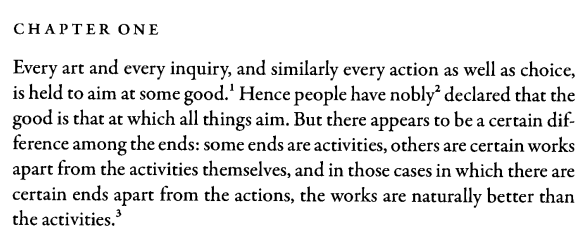
\includegraphics[width=0.85\textwidth]{aristotle2/page1.png}

    \bigskip
    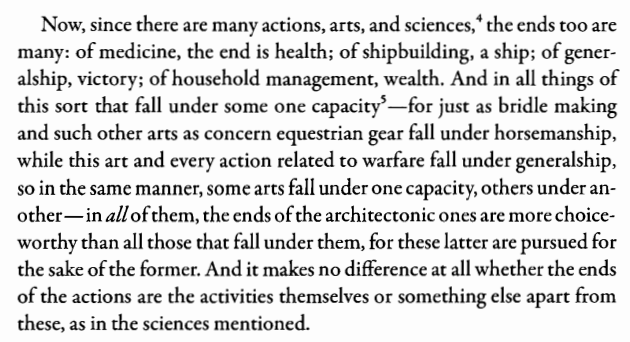
\includegraphics[width=0.85\textwidth]{aristotle2/page2.png}

    \bigskip
    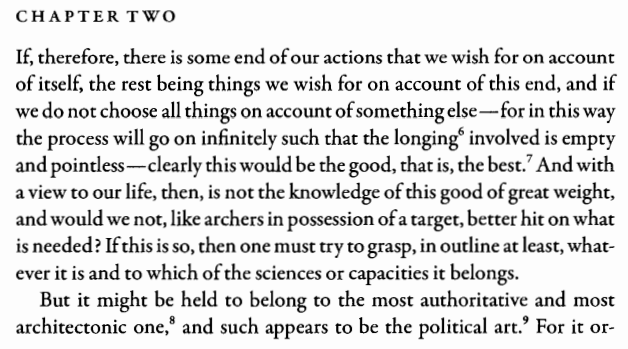
\includegraphics[width=0.85\textwidth]{aristotle2/page2.5.png}

    \bigskip
    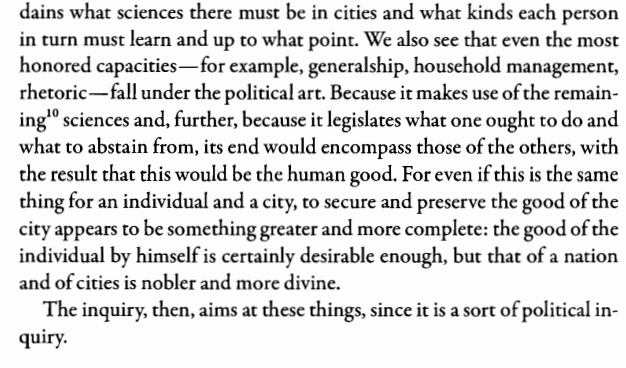
\includegraphics[width=0.85\textwidth]{aristotle2/page3.png}

    \captionof{figure}{Aristotle, Edition 2 --- a modern translation, cleaner typesetting.}
\end{center}

\bigskip
\begin{center}
    \begin{tabular}{lr}
        \toprule
        Metric & Value \\
        \midrule
        Word Error Rate      & 3.17\% \\
        Character Error Rate & 14.47\% \\
        Overall Similarity   & 84.79\% \\
        \bottomrule
    \end{tabular}
\end{center}
\bigskip

This is Qwen at its best, and the errors that remain are entirely cosmetic:

\begin{itemize}
    \item \textbf{Footnote markers flattened:} ``good.\textsuperscript{1}'' came back as
        ``good.1''; ``longing\textsuperscript{6}'' came back as
        ``longing\texttt{<sup>6</sup>}'' --- the model clearly recognized these as
        footnote markers, it just didn't render them as true Unicode superscripts.
    \item \textbf{One real word swap:} ``generalship,'' read as ``generals,'' --- a genuine
        misreading, but an isolated one.
\end{itemize}

No clauses were rewritten, no words were substituted with different meanings. The gap
between this edition and Edition~1 --- with the exact same model, the exact same task --- is
entirely attributable to scan/print quality. Clean, modern typesetting gets Qwen close to a
perfect transcription; older or messier print does not.

\section{\texorpdfstring{Arabic --- \textarabic{فريدة الدهر في طبقات قراء مصر}, Volume 1}{Arabic Source, Volume 1}}

\begin{center}
    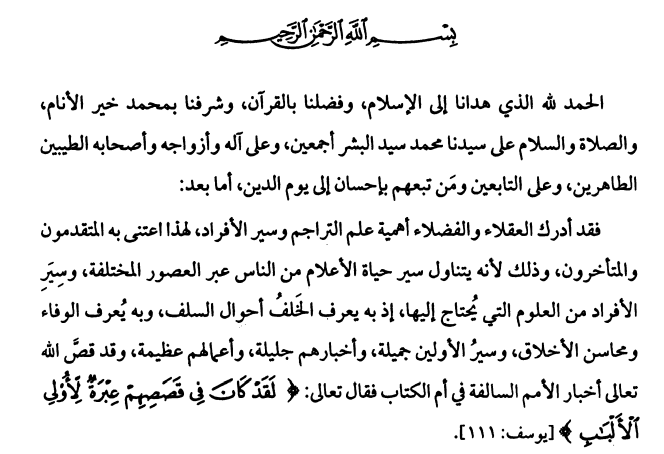
\includegraphics[width=0.85\textwidth]{arabic2/page.5.png}

    \bigskip
    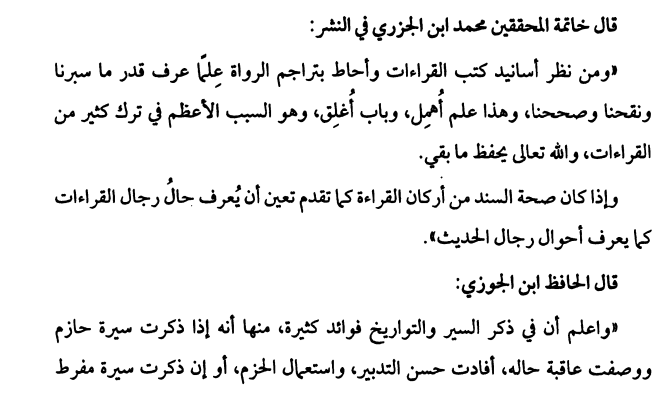
\includegraphics[width=0.85\textwidth]{arabic2/page1.png}

    \bigskip
    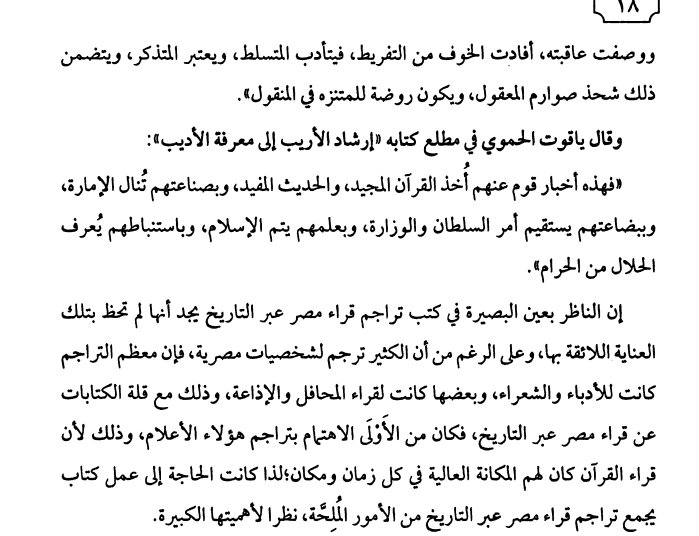
\includegraphics[width=0.85\textwidth]{arabic2/page1.5.png}

    \bigskip
    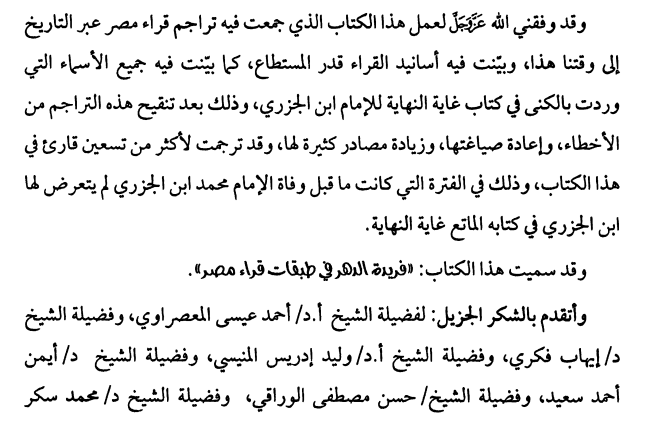
\includegraphics[width=0.85\textwidth]{arabic2/page2.png}

    \bigskip
    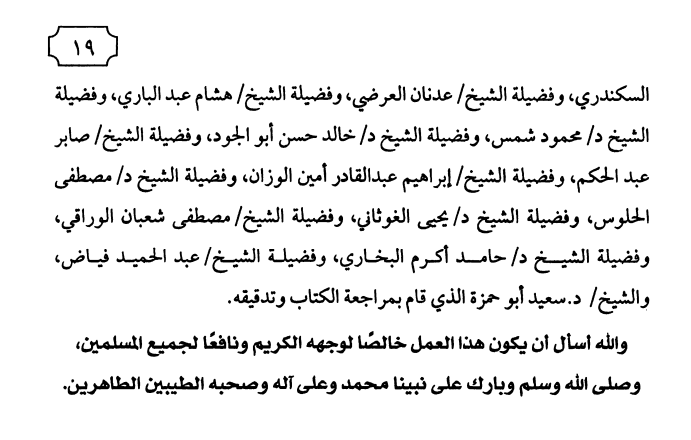
\includegraphics[width=0.85\textwidth]{arabic2/page2.5.png}

    \captionof{figure}{An Arabic biographical work on Egypt's Qur'an reciters, Volume 1.}
\end{center}

\bigskip
\begin{center}
    \begin{tabular}{lr}
        \toprule
        Metric & Value \\
        \midrule
        Word Error Rate      & 34.74\% \\
        Character Error Rate & 77.68\% \\
        Overall Similarity   & 22.65\% \\
        \bottomrule
    \end{tabular}
\end{center}
\bigskip

This is where Qwen's OCR clearly weakens, and it weakens in more than one way.

\textbf{On ordinary paragraph text}, it's readable but noticeably rougher than English.
Correct passages, like \textarabic{الحمد لله الذي هدانا إلى الإسلام}, come through exactly
right. But scattered throughout, diacritics (\emph{tashk\={\i}l}) get dropped or altered, and
words get swapped for similar-looking ones: \textarabic{وسِيَر} read as \textarabic{وسير};
\textarabic{أحوال} read as \textarabic{أخبار}. There's also at least one case of outright
invention on an otherwise ordinary line: the word \textarabic{قصَّ} (``narrated'') came back
as \textarabic{قص القرآن} --- the model added a word, ``the Qur'an,'' that isn't in the
source at all.

\textbf{On two specific pages, it broke down more seriously:}

\begin{itemize}
    \item The opening \emph{Bismillah} invocation, \textarabic{بِسْمِ اللهِ الرَّحْمَنِ
        الرَّحِيمِ}, came back as \textarabic{يُسۡنَـٰٓءُ ٱللَّهِ ٱلْخَزۡرِجِ} --- not a
        misreading of those words, but different words entirely.
    \item Further down the same page, a Qur'anic citation --- Surah Y\={u}suf 12:111,
        \textarabic{﴿ لَقَدْ كَانَ فِي قَصَصِهِمْ عِبْرَةٌ لِأُولِي الْأَلْبَابِ ﴾} --- was
        replaced with different Qur'anic-sounding phrasing altogether:
        \textarabic{﴿ قَدْ كَذَبَ الَّذِينَ فِي قُلُوبِهِم مَّرَضٌ لَّا يُؤْمِنُونَ ﴾},
        echoing the wording of other, unrelated verses about hypocrisy and disbelief. This
        is not a misreading of the printed characters --- it's the model substituting in
        different memorized religious text instead of reading what was actually on the
        page.
    \item A dense, small-font credits page came back with every word's Arabic letters in
        \textbf{reversed order} (e.g.\ \textarabic{الشيخ} rendered as its letters
        back-to-front). This was confirmed to be a consistent, reproducible failure ---
        rerunning that exact page twice at a deterministic setting produced identical,
        equally reversed output both times. This isn't the model guessing wrong; it's
        consistently misreading the script's letter order on that specific layout.
\end{itemize}

Put together, Arabic accuracy has two separate problems: ordinary transcription noise
(diacritics, similar-looking words, occasional small insertions), and outright hallucination
on top of it --- including, in one case, substituting in real but incorrect Qur'anic text
that was never on the page.

\section{The Takeaway}

Qwen3.5 is a genuinely strong OCR reader for English on a machine that can't run anything
bigger --- close to flawless on clean modern print, and still solidly usable on older,
archaic typesetting, with the caveat that it will occasionally smooth out awkward phrasing
into something more modern instead of transcribing it exactly. That caveat matters: this
model does not just misread text, it sometimes \emph{rewrites} it to sound more natural,
which is a fundamentally different and harder-to-catch kind of error than a simple typo.

Arabic is where that risk becomes serious. It's not just that the error rate roughly triples
--- it's that some of those errors are outright fabrications rather than misreadings, up to
and including swapping in different memorized religious phrasing in place of the Qur'anic
verse actually printed on the page. For a casual transcription job, Qwen3.5's Arabic OCR is
a reasonable starting point that will still need a careful human pass. For anything where
getting the exact text right actually matters --- religious texts chief among them --- it
cannot be trusted unsupervised, full stop.

\end{document}
